\subsection{Catégories \og SM \fg{}}\label{chapter-HTT_analysis-section-categorisation-SM}
\subsubsection{Définition des catégories}
Les catégories \CATsm, introduites dans les références~\cite{CMS-NOTE-2019-177,CMS-NOTE-2019-178}, sont construites dans le but d'étudier le boson de Higgs du \SM\ \higgs\ de masse \SI{125}{\GeV}.
Cette catégorisation est faite à l'aide d'un réseau de neurones dont l'objectif est de définir différentes catégories d'événements, chacune contenant un processus physique dominant.
Le principe des réseaux de neurones est abordé dans le chapitre~\refChML.
Le réseau utilisé est ici décrit succinctement, plus de détails sont disponibles dans la référence~\cite{CMS-NOTE-2019-178}.
%AN 2019/177 and 178
\paragraph{Structure du réseau de neurones}
Les principales variables d'entrée du réseau sont:
\begin{itemize}
\item les impulsions transverses des éléments du dilepton;
\item la masse transverse du dilepton dans le cas du canal \ele\mu\ ($\mT(\vpT^{\ele}+\vpT^{\mu},\vMET)$);
\item les impulsions transverses des deux principaux jets de l'événement;
\item le nombre de jets \Njets;
\item le nombre de jets de quarks~\quarkb\ \Nbjets;
\item la masse invariante du système des deux jets principaux \mjj;
\item la distance dans le plan $(\eta,\phi)$ entre les deux jets principaux \Detajj;
\item l'impulsion transverse totale des deux principaux jets de l'événement;
\item la masse du dilepton estimée par \SVFIT~\cite{SVFit_Bianchini_2014},
un estimateur de la masse d'une particule se désintégrant en paire de leptons~\tau\ par ajustement d'un profil de vraisemblance,
\msv;
\item la masse invariante du dilepton, \mvis;
\item l'impulsion transverse du dilepton, \pTvis.
\end{itemize}
Le réseau est constitué de deux couches cachées de 200 neurones chacune, complètement connectées.
Leur fonction d'activation est la tangente hyperbolique.
\par
Afin de permettre une catégorisation plus poussée qu'une simple discrimination signal ou bruit de fond, la couche de sortie du réseau contient autant de neurones que de catégories souhaitées.
Ce réseau fournit donc un vecteur et non un scalaire.
La fonction d'activation de ces neurones de sortie est la fonction exponentielle normalisée ou \emph{Softmax},
\begin{equation}
\mathit{Softmax}(\vec{z})_j = \frac{\exp(z_j)}{\sum_{k=1}^n \exp(z_k)}
\msep
j\in\set{1,\ldots,K}
\mend[,]
\end{equation}
chaque composante de ce vecteur est alors la probabilité que l'événement appartienne à la catégorie correspondante.
\paragraph{Catégories obtenues}
Pour chaque canal, deux catégories de signal existent visant chacune certains modes de production du boson de Higgs:
\begin{itemize}
\item \texttt{ggh}: production par fusion de gluons (\gluon\gluon\higgs);
\item \texttt{qqh}: production par fusion de bosons vecteurs (VBF) ou en association avec un boson (VH).
\end{itemize}
Ces modes de production sont introduits dans le chapitre~\refChMSSM.
\par
Une catégorie est également définie pour chacun des principaux bruits de fond, présentés dans la section~\ref{chapter-HTT_analysis-section-bg_estimation}.
La catégorie \CATemb\ doit correspondre aux données encapsulées décrites dans la section~\ref{chapter-HTT_analysis-section-bg_estimation-embedding}.
La catégorie \CATfake, quant à elle, doit contenir les événements décrits par la méthode des facteurs de faux présentée section~\ref{chapter-HTT_analysis-section-bg_estimation-FF_method}.
Pour les bruits de fond ayant une faible contribution ou étant peu différentiables d'autres bruits de fond, une catégorie \CATmisc\ est également définie.
Les différentes catégories ainsi possibles sont listées dans le tableau~\ref{tab-chapter-HTT_analysis-section-categorisation-SM-cats_recap}.
Le canal \tauh\tauh\ ne devant pas contenir d'électron ni de muons, les processus $\Zboson\to\ell\ell$ ($\ell\in\set{\ele,\mu}$), \ttbar\ et \Wjets\ contribuent peu au bruit de fond, c'est pourquoi il n'existe pas de catégories leur étant dédiées dans ce canal.
Ils sont donc associés à la catégorie \CATmisc\ pour le canal \tauh\tauh.
Celle-ci couvre donc les processus
$\Zboson\to\ell\ell$, \ttbar, \Wjets\ et Diboson dans le canal \tauh\tauh;
Diboson dans les canaux \mu\tauh\ et \ele\tauh;
$\Zboson\to\ell\ell$ et \Wjets\ dans le canal \ele\mu.
Les processus EWK $\Zboson\to LL$ et EWK $\Zboson\to \nu\nu$, introduits dans l'annexe~\refApHTTdatasets, sont également associés à la catégorie \CATmisc\ dans les canaux \tauh\tauh, \mu\tauh\ et \ele\tauh.
\begin{table}[h]
\centering
\begin{tabular}{ccccccc}
\toprule
Canal & \multicolumn{6}{l}{Catégories de bruit de fond possibles}\\
\midrule
\tauh\tauh & \CATemb & & & & \CATfake & \CATmisc \\
\mu\tauh & \CATemb & \CATzll & \CATttbar & & \CATfake & \CATmisc \\
\ele\tauh & \CATemb & \CATzll & \CATttbar & & \CATfake & \CATmisc \\
\ele\mu & \CATemb & & \CATttbar & \CATdib & \CATqcd & \CATmisc \\
\bottomrule
\end{tabular}
\caption{Catégories \CATsm\ de bruit de fond pour les quatre canaux considérés.}
\label{tab-chapter-HTT_analysis-section-categorisation-SM-cats_recap}
\end{table}
%Minor background processes like electroweak Z production or di-boson events which provide
%only small event numbers are collected in one category for remaining processes called ”misc”.
%Individual categories would raise problems to the training due to the small event numbers. In
%this collection they are at least respected in the training of the neural network such that they
%can’t migrate to the signal categories without increasing the training loss. Since there are no
%leptons in the τ h τ h decay channel, the yields of the Z → ll, tt̄, W + jets processes are rather
%small as well which is the reason that there are no dedicated categories in this channel. Instead
%these processes are associated with the misc category as well. In summary, the misc category
%covers Z → ll and W + jets in the eμ channel, di-Boson, single top and EWKZ in the eτ h and
%μτ h channel and Z → ll, tt̄, W + jets, di-Boson, single top and EWKZ in the τ h τ h channel.
\subsubsection{Variable discriminante}
\begin{figure}[p]
\centering

\subcaptionbox{Catégorie \CATxxh.}[.475\textwidth]
{\plotHTTshapes{mt_tot}{mssm_vs_sm_h125}{2017}{em}{1}{prefit}}
\hfill
\subcaptionbox{Catégorie \CATemb.}[.475\textwidth]
{\plotHTTshapes{mt_tot}{mssm_vs_sm_h125}{2017}{em}{20}{prefit_linear}}

\subcaptionbox{Catégorie \CATttbar.}[.475\textwidth]
{\plotHTTshapes{mt_tot}{mssm_vs_sm_h125}{2017}{em}{13}{prefit_linear}}
\hfill
\subcaptionbox{Catégorie \CATdib.}[.475\textwidth]
{\plotHTTshapes{mt_tot}{mssm_vs_sm_h125}{2017}{em}{19}{prefit_linear}}

\subcaptionbox{Catégorie \CATqcd.}[.475\textwidth]
{\plotHTTshapes{mt_tot}{mssm_vs_sm_h125}{2017}{em}{14}{prefit_linear}}
\hfill
\subcaptionbox{Catégorie \CATmisc.}[.475\textwidth]
{\plotHTTshapes{mt_tot}{mssm_vs_sm_h125}{2017}{em}{16}{prefit_linear}}

\caption[Distributions de \NNscore\ en 2017 dans le canal \ele\mu.]{Distributions de \NNscore\ en 2017 dans le canal \ele\mu.}
\label{fig-NNscore_distribs_exemple}
\end{figure}
Le réseau de neurones utilisé a pour but de classer les événements selon leur nature dans les différentes catégories définies précédemment.
De l'entraînement de ce réseau résultent les frontières entre les différentes catégories.
Les régions frontalières, \ie\ les régions de l'espace des phases dans lesquelles les événements ont de proches probabilités d'appartenir à deux catégories ou plus, sont ainsi délibérément fixées lors de l'entraînement et en dépendent.
Modifier les paramètres du réseau ou de l'entraînement mène ainsi à des migrations d'événements frontaliers d'une catégorie à une autre.
Or, ces derniers sont ceux dont la probabilité d'appartenir à une catégorie ne peut être grande, car dans ce cas ils seraient très caractéristiques de cette catégorie.
\par
Il est donc pertinent d'utiliser les valeurs de sortie du réseau pour définir une variable discriminante.
Le choix fait est d'utiliser la plus grande probabilité parmi celles données par le réseau, \ie\ la probabilité d'appartenir à la catégorie dans laquelle le réseau estime que cet événement fait partie.
Cette variable est dénommée \og score \fg{} et notée \NNscore.
À titre d'illustration, les distributions obtenues pour le canal \ele\mu\ en 2017 sont représentées en figure~\ref{fig-NNscore_distribs_exemple}.
\begin{wrapfigure}{R}{.45\textwidth}
\centering
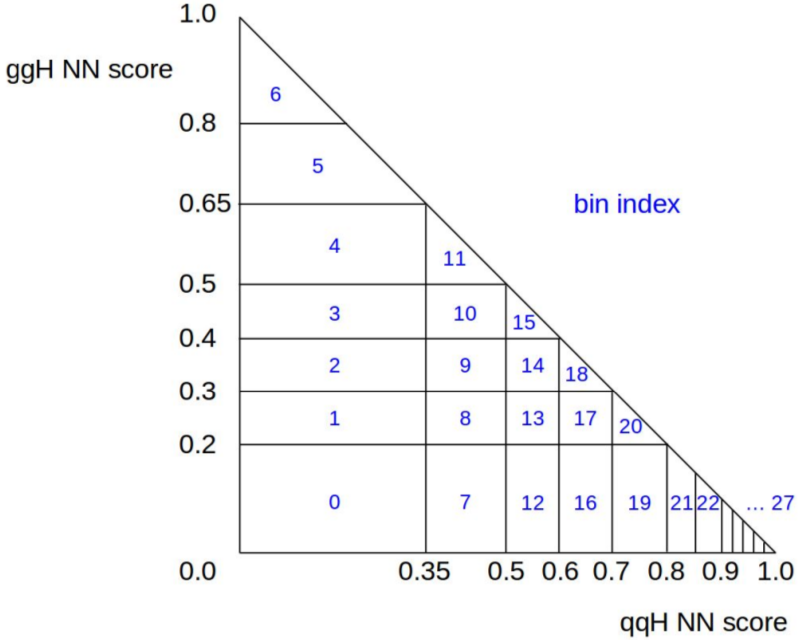
\includegraphics[width=.45\textwidth]{\PhDthesisdir/plots_and_images/from_CMS-NOTE-2019-177/fig67.png}
\caption[Réduction à une dimension de la catégorie \CATxxh.]{Réduction à une dimension de la catégorie \CATxxh~\cite{CMS-NOTE-2019-177}.}
\label{fig-67-CMS-NOTE-2019-177}
\end{wrapfigure}
\par
Certains événements de signal peuvent être difficilement classés dans une unique catégorie de signal, \texttt{ggh} ou \texttt{qqh}.
Dans ce cas, leurs scores sont bas pour ces catégories et ils
se retrouvent dans un segment de l'histogramme contenant d'avantage de bruit de fond
que s'ils avaient obtenu un score plus élevé.
Afin de limiter cet effet,
la solution trouvée~\cite{CMS-NOTE-2019-177} est de créer une catégorie globale $\CATxxh=\texttt{ggh} + \texttt{qqh}$.
Le score dans cette catégorie \CATxxh\ est alors bidimensionnel, chaque dimension correspondant à un des deux scores des catégories \texttt{ggh} et \texttt{qqh}.
Pour obtenir un histogramme à une dimension, une réduction est réalisée tel qu'illustré figure~\ref{fig-67-CMS-NOTE-2019-177}.
\par
La segmentation est à peu près uniforme en fonction du score \texttt{ggh}.
Aux bas scores \texttt{qqh}, elle est plus large à cause des larges contributions du bruit de fond ainsi que de la quantité réduite d'événements.
Aux hauts scores \texttt{qqh}, elle est plus fine car le signal y est fortement présent.
L'indice du \NNscore\ 2D ainsi obtenu est utilisé comme variable discriminante dans la catégorie \CATxxh.
Comme pour toutes les autres distributions, une resegmentation automatique est réalisée afin de s'assurer que chaque segment contienne au moins dix événements de bruit de fond.
C'est pourquoi les distributions peuvent montrer des segmentations variables, en particulier moins fines que celles initialement définies.
%The task of the neural net is to define regions of the phase space that are dominated by certain
%processes. The resulting boundaries between the categories, meaning the region where events
%are assigned similar and therefore low probabilities for two categories, are actually rather de-
%liberate and depend very much on the training parameters e.g. additional class weights. A
%variation of the parameters would cause migrations of these events between the categories.
%Therefore, it is important to use the actual values of the output nodes for further discrimina-
%tion and to sort events by it. Here we use the value of the largest probability, which was used to
%assign the category, for further discrimination within the same category. We call this quantity
%exclusive probability or just the NN score.